\section{Groups system}\label{sec:group-system}

One of the requirements for our app was that it should be possible to group repositories together.
The grouping is needed to view statistics for multiple repositories at once and also compare groups of repositories.
The grouping system should be also capable of controlling user access rights to different repositories.

Requirements for grouping system
\begin{itemize}
    \item It shall be possible to group both repositories and groups already consisting of repositories.
    \item Single repository may be possible of multiple groups.
    \item Group access can be limited to only viewing summary (group total).
    \item Granting user an access group subgroups and then removing it shall have no side effects. (Accesses to subgroups shall not be persisted)
\end{itemize}

As the groups may consist of both groups and repositories we decided to automatically create group for every repository.
This means now groups can only consist of zero or more other groups.
If we need te get the repository we can fetch all the group ids that are accessible and then query from repositories database by
comparing repositories group id against previously fetched ids;
To fetch group with all of its subgroups a recursive Structured Query Language (SQL) query was needed as the groups'
hierarchy formulates a tree like structure.
Our database provider PostgreSQL supports recursive queries so there were no technical problems with implementing it on SQL database.
A simplified version of our group system database tables can be seen of Figure~\ref{fig:group_system}

\begin{figure}[h]
    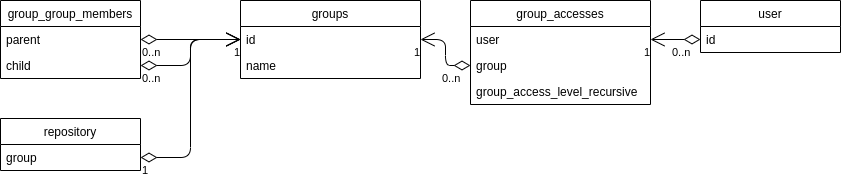
\includegraphics[width=\textwidth]{figures/group_system}
    \caption{Application groups system}
    \label{fig:group_system}
\end{figure}

This tree like groups' hierarchy allows us to easily give and take user access to any group.
If we want to change access from only parent group to also all subgroups access, we can simply toggle access\_level\_recursive
variable.
If we remove one particular group access, all other accesses remain in place, meaning that you some group was accessible
also via some other group access, you still have the access.

\section{Security}\label{sec:scurity}
Our application holds data, that shall not be visible to all client and therefore some kind of authentication and authorization methods are required.
For the data stored in Git notes we decided no extra security is required, as the time data isn't more sensitive than the actual code.
The security of source code stored in git repository is handled by a client himself and Git providers.
If they wish to have some more protection for git notes, they can configure it themselves.
We only provide the option to have notes only stored locally (not pushed to origin).

For the web application we need to implement our own security measures.
For most basic usage we have simple username and password authentication.
Accounts that only have password authentication are not authorized to access any groups nor repositories unless Admin user
explicitly gives them access to any.

To automatically get access to repositories you are contributor of you need to authenticate yourself via OAuth2 standard.
This way we can verify, that the user signing in to our application is the same user that has access to some git repository.

\subsection{OAuth2}\label{subsec:oauth2}
For OAuth2 authorization rocket\_oauth2 library is used, that follows RFC-6749 standard.
\cite{rocket-oauth2, oauth2}
We support authentication via Github.com, Gitlab.com, Bitbucket.org, Azure (Microsoft account) and TalTech gitlab server.
First three were chosen as they are the most common git server providers as of 2021.
Authentication via Microsoft was added as TalTech (and also numerous other universities / companies) use it and therefore
all students have already registered account there.
Also, it provides access to user emails, that can be later used to filter out user commits.
TalTech gitlab server was added, as the application is currently developed for TalTech and therefore it was a requirement
that everything shall also work on TalTech gitlab server.

From all OAuth2 providers at least user read access is required to get access to user emails.
For OAuth2 providers, that are also a Git server providers also permissions to read user repositories data is required.
User repositories data is used to give user automatically access to his own repositories and also display repositories
not currently tracked by gtm.
It also allows more easily adding automatic data collection to user repositories, as user can browse through
repositories from different git server providers.

\subsection{Adding tracking to repositories}\label{subsec:adding-tracking}
We have added three levels to view time data:
\begin{enumerate}
    \item Add tracking (locally), view data via gtm CLI app.
    \item Add tracking (locally), log data to commit messages.
    \item Add tracking, sync data to gtm Web App.
\end{enumerate}

All smaller level can be included while using higher level option.
Viewing data via CLI app is always possible, as it is the same app that is responsible for recording data.
This can be done both only locally or with pushing and pulling notes from remotes.
You can also add logging time spent to commit messages in both of the scenarios as it simply works on top of the already
existing system and only modifies commit message.
To use auto logging option you simply need to add --auto-log=\{gitlab/jira\} option when initiating tracking for repository.

To view data from web interface, some more steps are required.
User flow for making repository visible on gtm web application is shown on Figure~\ref{fig:add-tracking-user-flow}.

\begin{figure}[h]
    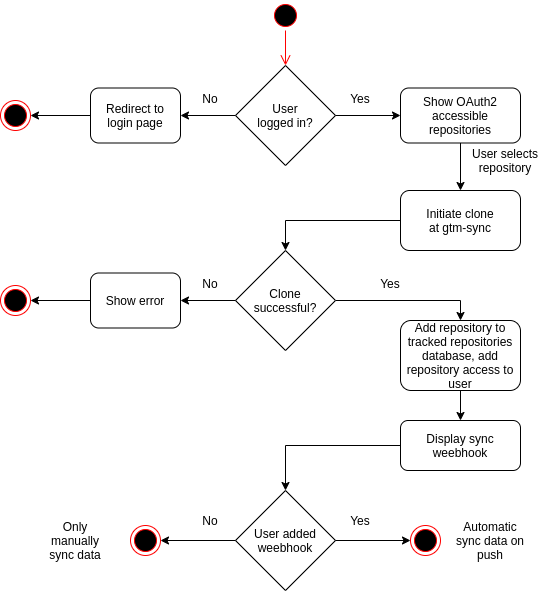
\includegraphics[width=\textwidth]{figures/add_repo_user_flow}
    \caption{Add tracking user flow}
    \label{fig:add-tracking-user-flow}
\end{figure}

Firstly, to have our sync client access the data, you cannot have time data only stored locally.
Then to add a repository, you need to have linked appropriate git server provider account via OAuth so that we can
verify that you have the access to repository.
After that you need to search for the repository from web interface and click add tracking button.
With that the tracking is technically added, but to also automatically sync time data on every push to remote,
you also need to add webhook.
